% Created by tikzDevice version 0.12.6 on 2024-10-23 10:55:45
% !TEX encoding = UTF-8 Unicode
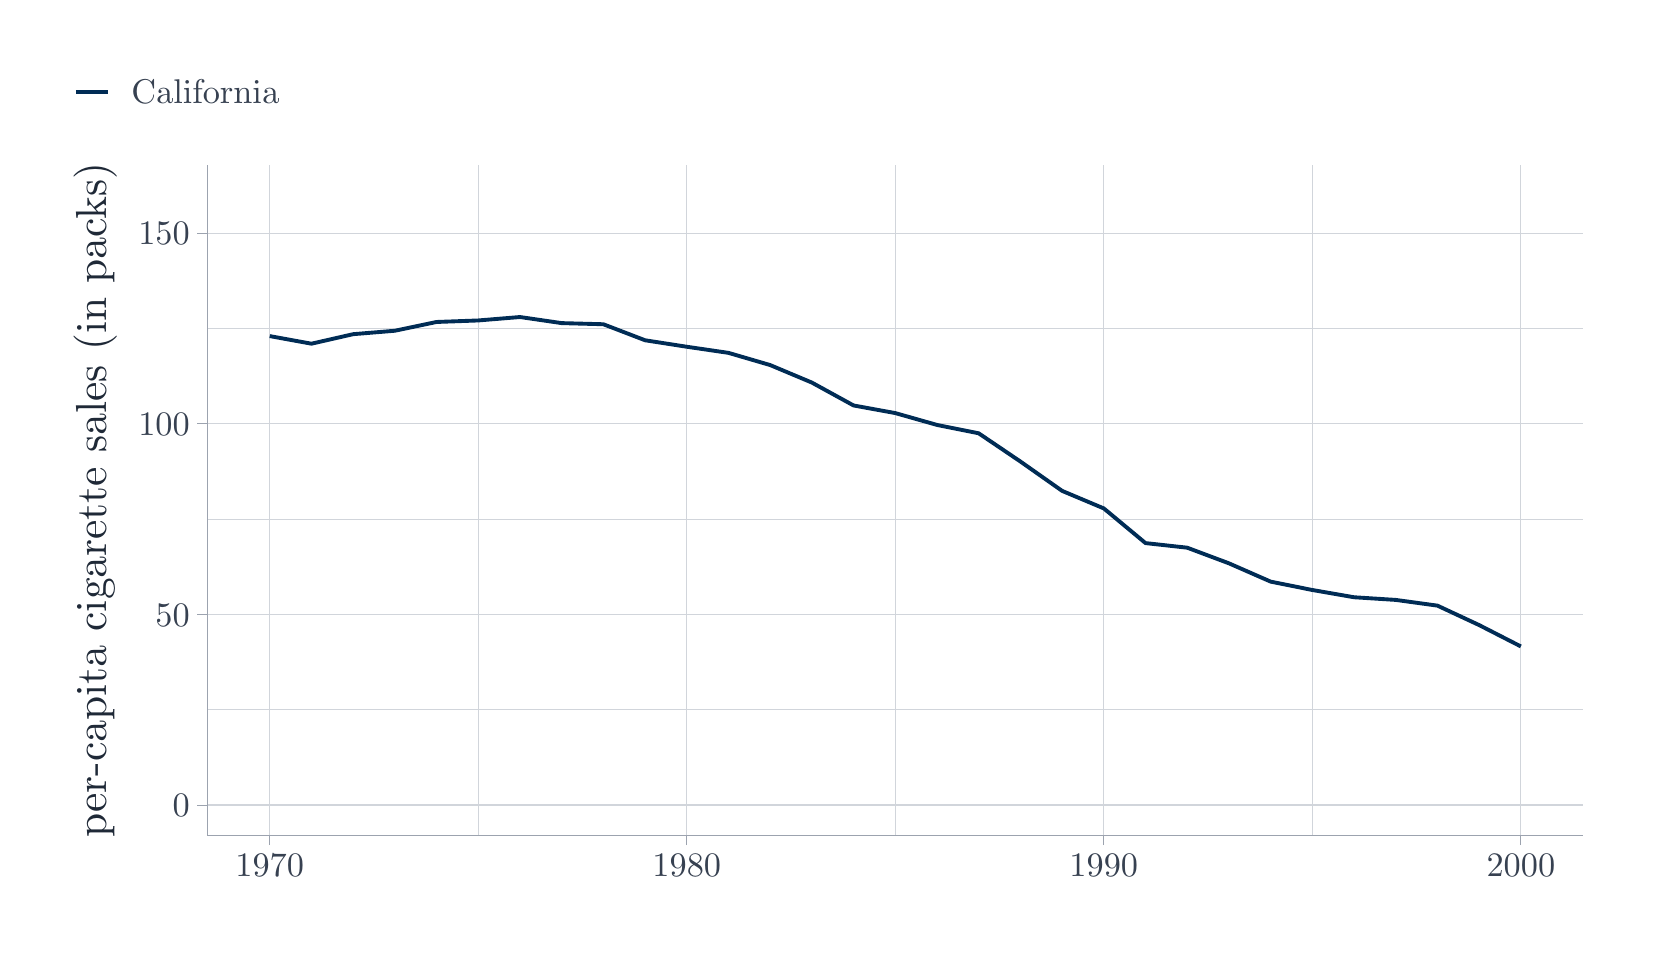
\begin{tikzpicture}[x=1pt,y=1pt]
\definecolor{fillColor}{RGB}{255,255,255}
\path[use as bounding box,fill=fillColor] (0,0) rectangle (578.16,325.21);
\begin{scope}
\path[clip] (  0.00,  0.00) rectangle (578.16,325.21);
\definecolor{drawColor}{RGB}{255,255,255}

\path[draw=drawColor,line width= 0.7pt,line join=round,line cap=round,fill=fillColor] (  0.00,  0.00) rectangle (578.16,325.21);
\end{scope}
\begin{scope}
\path[clip] ( 64.86, 33.29) rectangle (562.16,275.76);
\definecolor{drawColor}{RGB}{255,255,255}
\definecolor{fillColor}{RGB}{255,255,255}

\path[draw=drawColor,line width= 0.7pt,line join=round,line cap=round,fill=fillColor] ( 64.86, 33.29) rectangle (562.16,275.76);
\definecolor{drawColor}{RGB}{209,213,219}

\path[draw=drawColor,line width= 0.4pt,line join=round] ( 64.86, 78.75) --
	(562.16, 78.75);

\path[draw=drawColor,line width= 0.4pt,line join=round] ( 64.86,147.64) --
	(562.16,147.64);

\path[draw=drawColor,line width= 0.4pt,line join=round] ( 64.86,216.52) --
	(562.16,216.52);

\path[draw=drawColor,line width= 0.4pt,line join=round] (162.82, 33.29) --
	(162.82,275.76);

\path[draw=drawColor,line width= 0.4pt,line join=round] (313.51, 33.29) --
	(313.51,275.76);

\path[draw=drawColor,line width= 0.4pt,line join=round] (464.21, 33.29) --
	(464.21,275.76);

\path[draw=drawColor,line width= 0.4pt,line join=round] ( 64.86, 44.31) --
	(562.16, 44.31);

\path[draw=drawColor,line width= 0.4pt,line join=round] ( 64.86,113.19) --
	(562.16,113.19);

\path[draw=drawColor,line width= 0.4pt,line join=round] ( 64.86,182.08) --
	(562.16,182.08);

\path[draw=drawColor,line width= 0.4pt,line join=round] ( 64.86,250.96) --
	(562.16,250.96);

\path[draw=drawColor,line width= 0.4pt,line join=round] ( 87.47, 33.29) --
	( 87.47,275.76);

\path[draw=drawColor,line width= 0.4pt,line join=round] (238.16, 33.29) --
	(238.16,275.76);

\path[draw=drawColor,line width= 0.4pt,line join=round] (388.86, 33.29) --
	(388.86,275.76);

\path[draw=drawColor,line width= 0.4pt,line join=round] (539.56, 33.29) --
	(539.56,275.76);
\definecolor{drawColor}{RGB}{0,44,85}

\path[draw=drawColor,line width= 1.4pt,line join=round] ( 87.47,213.76) --
	(102.54,211.01) --
	(117.61,214.45) --
	(132.68,215.69) --
	(147.75,218.86) --
	(162.82,219.41) --
	(177.89,220.65) --
	(192.96,218.45) --
	(208.03,218.04) --
	(223.09,212.25) --
	(238.16,209.91) --
	(253.23,207.70) --
	(268.30,203.29) --
	(283.37,196.96) --
	(298.44,188.69) --
	(313.51,185.94) --
	(328.58,181.66) --
	(343.65,178.63) --
	(358.72,168.44) --
	(373.79,157.83) --
	(388.86,151.49) --
	(403.93,138.96) --
	(419.00,137.30) --
	(434.07,131.65) --
	(449.14,125.04) --
	(464.21,122.01) --
	(479.28,119.39) --
	(494.35,118.43) --
	(509.42,116.36) --
	(524.49,109.33) --
	(539.56,101.62);
\end{scope}
\begin{scope}
\path[clip] (  0.00,  0.00) rectangle (578.16,325.21);
\definecolor{drawColor}{RGB}{156,163,175}

\path[draw=drawColor,line width= 0.3pt,line join=round] ( 64.86, 33.29) --
	( 64.86,275.76);
\end{scope}
\begin{scope}
\path[clip] (  0.00,  0.00) rectangle (578.16,325.21);
\definecolor{drawColor}{RGB}{55,65,81}

\node[text=drawColor,anchor=base east,inner sep=0pt, outer sep=0pt, scale=  1.24] at ( 58.56, 40.02) {0};

\node[text=drawColor,anchor=base east,inner sep=0pt, outer sep=0pt, scale=  1.24] at ( 58.56,108.91) {50};

\node[text=drawColor,anchor=base east,inner sep=0pt, outer sep=0pt, scale=  1.24] at ( 58.56,177.79) {100};

\node[text=drawColor,anchor=base east,inner sep=0pt, outer sep=0pt, scale=  1.24] at ( 58.56,246.68) {150};
\end{scope}
\begin{scope}
\path[clip] (  0.00,  0.00) rectangle (578.16,325.21);
\definecolor{drawColor}{RGB}{156,163,175}

\path[draw=drawColor,line width= 0.3pt,line join=round] ( 61.36, 44.31) --
	( 64.86, 44.31);

\path[draw=drawColor,line width= 0.3pt,line join=round] ( 61.36,113.19) --
	( 64.86,113.19);

\path[draw=drawColor,line width= 0.3pt,line join=round] ( 61.36,182.08) --
	( 64.86,182.08);

\path[draw=drawColor,line width= 0.3pt,line join=round] ( 61.36,250.96) --
	( 64.86,250.96);
\end{scope}
\begin{scope}
\path[clip] (  0.00,  0.00) rectangle (578.16,325.21);
\definecolor{drawColor}{RGB}{156,163,175}

\path[draw=drawColor,line width= 0.3pt,line join=round] ( 64.86, 33.29) --
	(562.16, 33.29);
\end{scope}
\begin{scope}
\path[clip] (  0.00,  0.00) rectangle (578.16,325.21);
\definecolor{drawColor}{RGB}{156,163,175}

\path[draw=drawColor,line width= 0.3pt,line join=round] ( 87.47, 29.79) --
	( 87.47, 33.29);

\path[draw=drawColor,line width= 0.3pt,line join=round] (238.16, 29.79) --
	(238.16, 33.29);

\path[draw=drawColor,line width= 0.3pt,line join=round] (388.86, 29.79) --
	(388.86, 33.29);

\path[draw=drawColor,line width= 0.3pt,line join=round] (539.56, 29.79) --
	(539.56, 33.29);
\end{scope}
\begin{scope}
\path[clip] (  0.00,  0.00) rectangle (578.16,325.21);
\definecolor{drawColor}{RGB}{55,65,81}

\node[text=drawColor,anchor=base,inner sep=0pt, outer sep=0pt, scale=  1.24] at ( 87.47, 18.42) {1970};

\node[text=drawColor,anchor=base,inner sep=0pt, outer sep=0pt, scale=  1.24] at (238.16, 18.42) {1980};

\node[text=drawColor,anchor=base,inner sep=0pt, outer sep=0pt, scale=  1.24] at (388.86, 18.42) {1990};

\node[text=drawColor,anchor=base,inner sep=0pt, outer sep=0pt, scale=  1.24] at (539.56, 18.42) {2000};
\end{scope}
\begin{scope}
\path[clip] (  0.00,  0.00) rectangle (578.16,325.21);
\definecolor{drawColor}{RGB}{31,41,55}

\node[text=drawColor,rotate= 90.00,anchor=base,inner sep=0pt, outer sep=0pt, scale=  1.57] at ( 28.38,154.52) {per-capita cigarette sales (in packs)};
\end{scope}
\begin{scope}
\path[clip] (  0.00,  0.00) rectangle (578.16,325.21);
\definecolor{drawColor}{RGB}{255,255,255}
\definecolor{fillColor}{RGB}{255,255,255}

\path[draw=drawColor,line width= 0.7pt,line join=round,line cap=round,fill=fillColor] ( 16.00,289.76) rectangle ( 91.04,309.22);
\end{scope}
\begin{scope}
\path[clip] (  0.00,  0.00) rectangle (578.16,325.21);
\definecolor{drawColor}{RGB}{255,255,255}
\definecolor{fillColor}{RGB}{255,255,255}

\path[draw=drawColor,line width= 0.7pt,line join=round,line cap=round,fill=fillColor] ( 16.00,294.76) rectangle ( 30.45,309.22);
\end{scope}
\begin{scope}
\path[clip] (  0.00,  0.00) rectangle (578.16,325.21);
\definecolor{drawColor}{RGB}{0,44,85}

\path[draw=drawColor,line width= 1.4pt,line join=round] ( 17.45,301.99) -- ( 29.01,301.99);
\end{scope}
\begin{scope}
\path[clip] (  0.00,  0.00) rectangle (578.16,325.21);
\definecolor{drawColor}{RGB}{55,65,81}

\node[text=drawColor,anchor=base west,inner sep=0pt, outer sep=0pt, scale=  1.24] at ( 37.45,297.70) {California};
\end{scope}
\end{tikzpicture}
